\documentclass{article}

\usepackage[utf8]{inputenc}
\usepackage[spanish]{babel}

\usepackage{caratula}

\usepackage{subcaption}
\usepackage{graphicx}
\usepackage{subfig}
\usepackage{dirtytalk}
\usepackage{enumerate}
\graphicspath{ {images/} }

\usepackage{amssymb}
\usepackage{mathtools}
\usepackage{amsmath}
\usepackage{amsthm}

\usepackage{algorithm}
\usepackage{algpseudocode}
\usepackage{listingsutf8}
\usepackage{float}
\floatplacement{figure}{h!}
\lstset{
    breaklines=true,
    postbreak=\raisebox{0ex}[0ex][0ex]{\ensuremath{\color{red}\hookrightarrow\space}}
}

\usepackage{geometry}
\usepackage{fixltx2e}
\usepackage{wrapfig}
\usepackage{cite}
\usepackage{dsfont}

\usepackage[space]{grffile}

\geometry{
 a4paper,
 total={210mm,297mm},
 left=30mm,
 right=30mm,
 top=30mm,
 bottom=30mm,
 }

 \newtheorem{theorem}{Teorema}[section]
 \newtheorem{corollary}{Corolario}[theorem]
\newtheorem{lemma}{Lema}[theorem]

 \theoremstyle{definition}
 \newtheorem{definition}{Definición}[section]

 \theoremstyle{remark}
 \newtheorem*{remark}{Observación}

\usepackage[dvipsnames]{xcolor}

\begin{document}
% Estos comandos deben ir antes del \maketitle
\materia{Teoria de Lenguajes} % obligatorio

\titulo{Trabajo Práctico}
\subtitulo{Dibu: Gráficos vectoriales para niños}
\grupo{}

\integrante{Julián Bayardo}{850/13}{julian@bayardo.com.ar} % obligatorio
\integrante{Christian Cuneo}{755/13}{chriscuneo93@gmail.com} % obligatorio

\maketitle

\pagebreak

\tableofcontents

\pagebreak

\section{Introducción}
Se nos presenta un lenguaje con una estructura especifica y se nos pide que generemos un analizador léxico y un analizador sintáctico para poder decidir la pertenencia de una cadena a este lenguaje, y si es así, obtener la estructura de esta cadena.
El lexer nos va a permitir reconocer los elementos del lenguaje que se encuentran en la cadena. Y el parser (analizador sintáctico) nos va a indicar si lo que fue escrito con esos elementos tiene sentido (cumple la estructura del lenguaje).

En nuestro caso el lenguaje describe una forma de construir un conjunto figuras geométricas que van a componer un gráfico. Para lograr esto el lenguaje consiste en una serie de instrucciones que van a definir distintos tipos de figuras y el gráfico en su totalidad.

Luego buscamos también lograr transformar la estructura de la cadena parseada en una cadena valida del lenguaje SVG (que funciona sobre xml)

Los dos son problemas separados, pero básicamente consiste en obtener la estructura de la cadena de entrada (si esta es valida) y transformarla elemento por elemento en una cadena valida SVG.

\section{Gramática}
La gramática que generamos que describe todas las cadenas de este lenguaje es la siguiente:

\begin{itemize}
  \item $S \rightarrow statement$
  \item $statement \rightarrow expression$
  \item $statement \rightarrow statement\, expression$
  \item $expression \rightarrow IDENTIFIER\, key\_value\_list$
  \item $key\_value\_list \rightarrow key\_value\_entry\, COMMA\, key\_value\_list$
  \item $key\_value\_list \rightarrow key\_value\_entry$
  \item $key\_value\_entry \rightarrow KEY\, EQUALS\, value$
  \item $value \rightarrow STRING$
  \item $value \rightarrow NUMBER$
  \item $value \rightarrow LPAREN\, value\, COMMA\, value\, RPAREN$
  \item $value \rightarrow LBRACKET\, array\, RBRACKET$
  \item $array \rightarrow value$
  \item $array \rightarrow value\, COMMA\, array$
\end{itemize}

Donde los elementos en mayúscula son símbolos terminales que matchean con las siguientes expresiones regulares:

\begin{lstlisting}  
  IDENTIFIER = (size|rectangle|line|circle|ellipse|polyline|polygon|text)
  STRING = \"([^\\\n]|(\\.))*?(?<!\\)"
  KEY = \w[\w\d_-]*
  COMMA = ,
  EQUALS = =
  LBRACKET = \[
  RBRACKET = \]
  LPAREN = \(
  RPAREN = \)
  NUMBER = \d+
\end{lstlisting}

Podemos observar que la gramática definida no es LL(1) por las reglas de statement, key\_value\_list y array; además, no es LR(0) por tener varios conflictos shift reduce: uno ocasionado por la regla $S \rightarrow statement$, otro ocasionado por la regla $key\_value\_list \rightarrow key\_value\_entry$, y otro por la regla $array \rightarrow value$. Puede verse (o bien haciendo el autómata a mano, o bien a través de PLY, o bien utilizando una herramienta como el Grammophone), que la gramática es SLR(1) (y por ende también LALR y LR(1)). De hecho, nuestra solución utiliza el método SLR de PLY.

\section{Solución}
La solución se realizo utilizando el esqueleto provisto por la cátedra, quiere decir usando $python$ y la librería $ply$ de ese lenguaje.
Para correr el parser se utilizo el $Notebook$ de $Jupyter$ dado por la cátedra pero levemente modificado (se encuentra en el código fuente)

El código se encuentra también en el informe pero adjuntado al final del mismo para una mayor comodidad de lectura.

Para la implementación utilizamos como referencia el código de los distintos lexers y parsers provistos por la cátedra.
No nos surgieron problemas reales al implementar la solución mas que entender como funcionaba la librería utilizada.
Tuvimos problemas simplemente al querer obtener la fila actual al estar parseando una subexpresión, mas que nada para levantar errores que sean auto explicativos y concisos, pero otra vez, fue mas un problema de entender como funcionaba la librería $ply$.

También decidimos levantar errores semánticos detallados cuando la cadena no cumple la semántica del lenguaje (osea, que quizás lexicografica y sintácticamente es correcta pero no tiene sentido).

\section{Como usar nuestro parser}
Como indicamos previamente la forma mas fácil de utilizarlo es a través del $Notebook$ de $Jupyter$.
Utilizamos $Python$ $3.5$ para implementar y correr el código. Luego los requerimientos están especificados en el archivo $requirements.txt$ por lo tanto se pueden instalar fácilmente con $pip$

En el $notebook$ $dibu.ipynb$ dejamos se encuentran ejemplos de como correr la herramienta.

Tambien se puede correr desde la carpeta principal del source de la forma: \\
$python3\, -m\, dibu.parser\,  '\#\#\#CADENA\, A\, PARSEAR\#\#\#'$

\section{Casos de prueba}

\subsection{Círculos superpuestos}

\textbf{Input:}
\begin{lstlisting}
size height=100, width=100
circle center=(50, 50), radius=50, fill="red"
circle center=(50, 50), radius=25, fill="black"
\end{lstlisting}

\textbf{Output:}


\includegraphics{1.png}

\subsection{Cuadrado con polígonos internos}

\textbf{Input:}
\begin{lstlisting}
size height=200, width=200
rectangle upper_left=(0,0), width=200, height=200,fill="yellow"
polygon points=[(0,0), (50, 50), (0, 100)], stroke="black", stroke-width=3, fill="none"
polygon points=[(0,0), (50, 50), (100, 0)], stroke="black", stroke-width=3, fill="none"
polygon points=[(0, 100), (50, 150), (0, 200)],stroke="black", stroke-width=3, fill="none"
polygon points=[(0, 200), (50, 150), (100, 200)],stroke="black", stroke-width=3, fill="none"
polygon points=[(100, 200), (150, 150), (200,200)], stroke="black", stroke-width=3, fill="none"
polygon points=[(200, 200), (150, 150), (200,100)], stroke="black", stroke-width=3, fill="none"
polygon points=[(200, 100), (150, 50), (200, 0)],stroke="black", stroke-width=3, fill="none"
polygon points=[(200, 0), (150, 50), (100, 0)],stroke="black", stroke-width=3, fill="none"
\end{lstlisting}

\textbf{Output:}


\includegraphics{2.png}

\subsection{Error semántico (size definido 2 veces)}

\textbf{Input:}
\begin{lstlisting}
size height=200, width=200
rectangle upper_left=(0,0), width=200, height=200, fill="yellow"
size height=200, width=200
\end{lstlisting}

\textbf{Output:}

\begin{lstlisting}[language=Python]
    SemanticException: Line 3: Size defined twice.
\end{lstlisting}

\subsection{Cuadrado con puntas redondeadas y poco opaco}

\textbf{Input:}
\begin{lstlisting}
size width=400, height=180
rectangle upper_left=(50,20), rx=20, ry=20, width=150, height=150, style="fill:red;stroke:black;stroke-width:5;opacity:0.5"
\end{lstlisting}

\textbf{Output:}

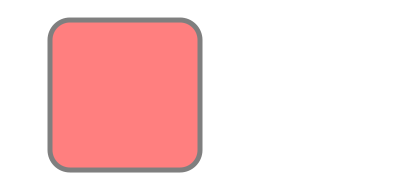
\includegraphics{4.png}

\subsection{Cuadrado con circulos adentro y texto abajo}

\textbf{Input:}
\begin{lstlisting}
size width=400, height=300
rectangle upper_left=(50,20), rx=20, ry=20, width=150, height=150, style="fill:red;stroke:black;stroke-width:5;opacity:0.5"
circle center=(125, 95), radius=50, fill="red"
circle center=(125, 95), radius=25, fill="black"
text at=(10, 200), t="Metiste un cutucuchillo y te pode queda lectrificada loca
\end{lstlisting}

\textbf{Output:}


\includegraphics{5.png}

\subsection{Error semántico parámetro no existe para rectangulo}

\textbf{Input:}
\begin{lstlisting}
size width=400, height=180
rectangle mama=(50,20)
\end{lstlisting}

\textbf{Output:}
\begin{lstlisting}[language=Python]
    SemanticException: Line 1: Parameters ['upper_left'] need to be defined for rectangle
\end{lstlisting}

\subsection{Error sintáctico identificador token no existe}

\textbf{Input:}
\begin{lstlisting}
size width=400, height=180
rectangsdale upper_left=(50,20)
\end{lstlisting}

\textbf{Output:}
\begin{lstlisting}[language=Python]
    Exception: [Syntax error]
    type:KEY
    value:rectangsdale
    line:2
    position:31
\end{lstlisting}

\section{Conclusiones}
Los resultados fueron correctos. Nos tomamos la libertad de agregar el parámetro opcional $rx$ y $ry$ al $rectangle$ y $style$ a todos para ver resultados mas interesantes. 

Encontramos interesante implementar el lexer y parser ya que nos deja ver de forma muy clara como se utiliza una gramática para ver si una cadena pertenece a un lenguaje.
\pagebreak

\section{Código}

\subsection{Parser}
\lstinputlisting[language=Python]{code/parser.py}

\subsection{Reglas del lexer}
\lstinputlisting[language=Python]{code/lexer_rules.py}

\subsection{Reglas del parser}
\lstinputlisting[language=Python]{code/parser_rules.py}

\end{document}
